%-----------------------------------LICENSE------------------------------------%
%   This file is part of tikz_figures.                                         %
%                                                                              %
%   tikz_figures is free software: you can redistribute it and/or              %
%   modify it it under the terms of the GNU General Public License as          %
%   published by the Free Software Foundation, either version 3 of the         %
%   License, or (at your option) any later version.                            %
%                                                                              %
%   tikz_figures is distributed in the hope that it will be useful,            %
%   but WITHOUT ANY WARRANTY; without even the implied warranty of             %
%   MERCHANTABILITY or FITNESS FOR A PARTICULAR PURPOSE.  See the              %
%   GNU General Public License for more details.                               %
%                                                                              %
%   You should have received a copy of the GNU General Public License along    %
%   with tikz_figures.  If not, see <https://www.gnu.org/licenses/>.           %
%------------------------------------------------------------------------------%

% Use the standalone class for displaying the tikz image on a small PDF.
\documentclass[crop, tikz]{standalone}

% Import the tikz package to use for the drawing.
\usepackage{tikz}

% Tikz packages used.
\usetikzlibrary{arrows.meta}

% Begin the document.
\begin{document}

    % Begin the drawing.
    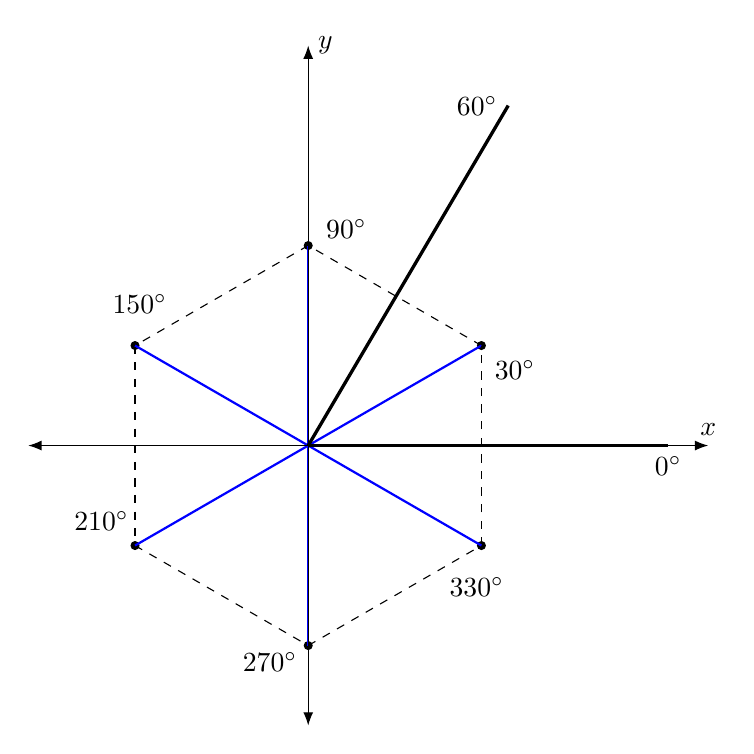
\begin{tikzpicture}[> = Latex]

        % Point for the origin.
        \coordinate (O) at (0.0in, 0.0in);

        % Loop through each angle in the hexagon.
        \foreach[%
            evaluate = {\phi = int(\theta + 60)},
            evaluate = {\labelang = int(\theta - 10)}
        ] \theta in {30, 90, ..., 330}{

            % Coordinate for the current and next point, and for the label.
            \coordinate (P0) at (\theta:1in);
            \coordinate (P1) at (\phi:1in);
            \coordinate (LABEL) at (\labelang:1.1in);

            % Mark at dot at the current point.
            \filldraw (P0) circle (0.5mm);

            % Dashed line connecting this one to the next.
            \draw[dashed] (P0) to (P1);

            % Blue line for the "spoke" from the origin to the point.
            \draw[thick, blue] (O) to (P0);

            % Label the angle, in degrees.
            \node at (LABEL) {$\theta^{\circ}$};
        }

        % Draw the coordinate axes.
        \draw[<->] (-1.4in, 0.0in) to (2.0in, 0.0in) node [above] {$x$};
        \draw[<->] (0.0in, -1.4in) to (0.0in, 2.0in) node [right] {$y$};

        % Angle marker for the origin, and the line at 60 degrees.
        \draw[very thick] (O) to (1.8in, 0.0in) node [below] {$0^{\circ}$};
        \draw[very thick] (O) to (1.0in, 1.7in) node [left] {$60^{\circ}$};
    \end{tikzpicture}
\end{document}
